\subsection{Business Logic Layer}
ViewModels ligger som en mellemting mellem business logic layer og presentation layer. Der foregår en binding til fra viewsne til dataen i viewmodels.

\subsection{Business Logic Layer}
ViewModels ligger som en mellemting mellem business logic layer og presentation layer. Der foregår en binding til fra viewsne til dataen i viewmodels.

\subsubsection*{Viewmodel kommunikation}
Alle view startes fra MainViewViewModel, som invidviduelt starter deres egen viewmodel. Det betyder at det ville være nødvendigt at lave data globalt for at kunne arbejde på den samme data, som f.eks. kategorier og de individuelle produkter i disse. \\
For at løse dette, har vi valgt at bruge Prism EventAggregator~\cite{PRISM}, som tillader os at kommu-nikere på tværs af viewmodels. Når MainViewViewModel startes, subscriber den på en række forskellige events, som bliver rasied når følgende vinduer bliver loaded:

\begin{itemize}
\item AddProductWindow
\item AddCategoryWindow
\item EditProductWindow
\item EditCategoryWindow
\item DeleteCategoryWindow
\end{itemize}


MainWindowViewModel har da en metode for hver af disse events, som bliver kaldt når disse events bliver rasied. Når dette sker publisher MainWindowViewModel så et event, svarende til det vindue der er blevet loaded. Eksempelvis vil AddCategory’s eventhandler publishe et event som AddCate-goryWindow subscriber på, med alle de nuværende kategorier som en parameter.\\

På denne måde undgår vi da, at der skal sendes data ind i et view, og videre ned i en viewmodel. Hvis der er brug for mere end en parameter, eksempelvis EditProduct som skal bruge fire parametre, er det nødvendigt at lave sin egen parameter-type for dette  (Backend.Models.Events : Parameters).

\begin{figure}[!h]
    \centering
    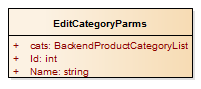
\includegraphics[width=0.3\textwidth]{Systemdesign/backend/Images/parms.png}
    \caption{Eksempel på parametermodel, der i dette tilfælde er til når EditProductViewet bliver loaded}
    \label{fig:editparms}
\end{figure}



\subsubsection{Viewmodel kommunikation}
\label{viewcomm}
Alle view startes fra MainViewViewModel, som invidviduelt starter deres egen viewmodel. Det betyder at det ville være nødvendigt at lave data globalt for at kunne arbejde på den samme data, som f.eks. kategorier og de individuelle produkter i disse. \\
For at løse dette, er det valgt at bruge Prism EventAggregator~\cite{PRISM}, som tillader at kommunikere på tværs af viewmodels. Når MainViewViewModel startes, subscriber den på en række forskellige events, som bliver rasied når følgende vinduer bliver åbnet:

\begin{itemize}
\item AddProductWindow
\item AddCategoryWindow
\item EditProductWindow
\item EditCategoryWindow
\item DeleteCategoryWindow
\end{itemize}


MainWindowViewModel har da en metode for hver af disse events, som bliver kaldt når disse vinduer åbnes. Når dette sker publisher MainWindowViewModel så et event, som indeholder data som den pågældende viewmodel skal bruge. Eksempelvis vil AddCategory’s eventhandler publishe et event som AddCategoryWindow subscriber på, med en liste over de nuværende kategorier som en parameter.\\

På denne måde undgås, at der skal sendes data ind i et view, og videre ned i en viewmodel. Hvis der er brug for mere end en parameter, eksempelvis EditProduct som skal bruge fire parametre, er det nødvendigt at lave sin egen parameter-type for dette  (Backend.Models.Events : Parameters).

\begin{figure}[H]
    \centering
    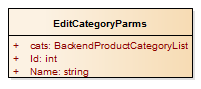
\includegraphics[width=0.3\textwidth]{Systemdesign/backend/Images/parms.png}
    \caption{Datamodel der bruges ved kommunikation mellem viewmodels}
    \label{fig:editparms}
\end{figure}

Figur \ref{fig:editparms} viser en model der indeholder parametre, som skal bruges når der skal sendes en event til EditCategoryWindow, når dette view bliver loadet. Dette er et eksempel på en af de klasser der bruges til at sende data til en viewmodel fra en anden, ved hjælp af EventAggregatoren.\\

På figur \ref{fig:viewmodelcomm} er der ved hjælp af et sekvensdiagram vist, hvordan viewmodels kommunikerer igennem EventAggregatoren.

\begin{figure}[H]
	\centering
	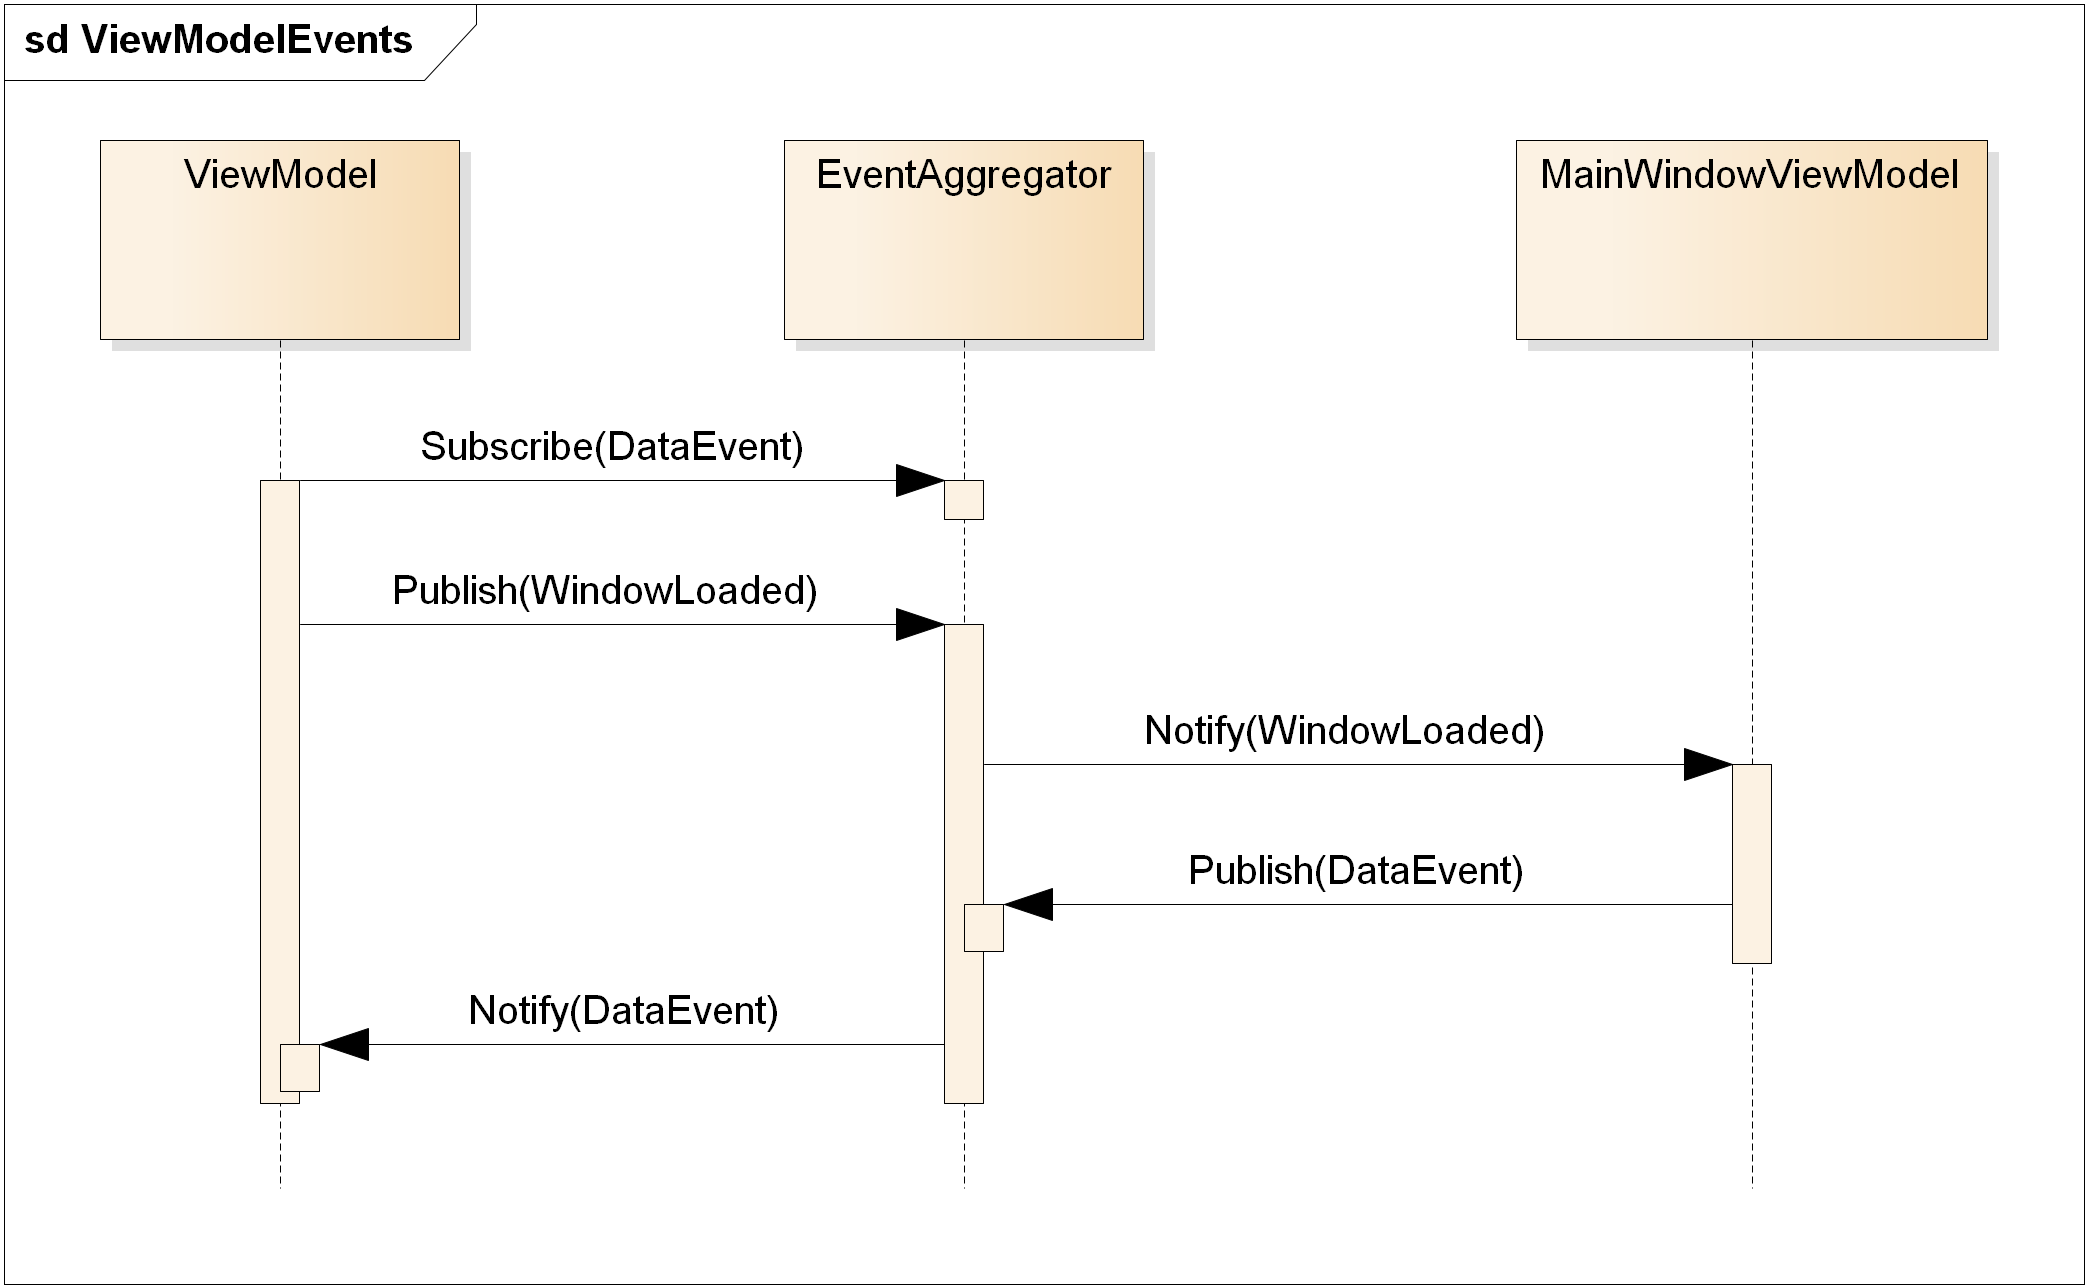
\includegraphics[width=1\textwidth]{Systemdesign/backend/Images/ViewModelEvents}
	\caption{Kommunikation mellem viewmodels}
	\label{fig:viewmodelcomm}
\end{figure}

For at forstå diagrammet på figur \ref{fig:viewmodelcomm} kræves lidt forklaring af de forskellige elementer i diagrammet.\\
\textit{ViewModel} repræsenterer en hvilken som helst viewmodel der åbnes.\\
\textit{DataEvent} er en generisk repræsentation af et event, som er specifikt til den pågældende viewmodel. Denne event bliver raised med data som den pågældende viewmodel skal bruge.
\textit{WindowLoaded} er den event MainWindowViewModel subscriber på, for at blive notifikeret, når viewmodelen oprettes.

For at tage et konkret eksempel bruges \textit{EditCategoryWindow}. Denne har en \textit{EditCategoryViewModel}. Når denne viewmodel oprettes subscriber viewmodelen på et \textit{NewEditCategoryData} event. Efterfølgende publisher viewmodelen \textit{EditCategoryWindowLoaded} event, som MainWindowViewModel allerede har subscribet på, da MainWindowViewModel blev oprettet. Derfor bliver MainWindowViewModel notifikeret om event, og handler derfor eventen. Handling af eventet er blot at publishe en \textit{NewEditCategoryData} event, med den korrekte data i. I dette tilfælde ville det være \textit{EditCategoryParms} der blev sendt med som parameter til eventen. Da EditCategoryViewModel har subscribet på denne event vil viewmodelen modtage den data der skal bruges i EditCategoryViewModel.